\section{Automatisierung eines Geschäftsprozesses}
\label{chap:automation}

In diesem Kapitel wird erläutert, warum es für ein Unternehmen überhaupt sinnvoll ist, einen Geschäftsprozess zu automatisieren und welche Risiken damit einhergehen. Es wird beschrieben, warum die künstliche Intelligenz bei der Automatisierung eines Geschäftsprozesses zur Anwendung kommt. Weiter werden Beispiele der Anwendung von künstlicher Intelligenz zur Automatisierung beschrieben und auf Erfolg und Probleme analysiert. Zum Schluss wird ein Einstig in die Thematik der künstlichen Intelligenz gewährt, welcher die Grundlage für das Fallbeispiel im nächsten Kapitel bildet.

\todo[inline, color=igloo]{Evtl. etwas zur Ethik sagen. Mit der rasanten Industrie 4.0 könnten tausende Menschen Arbeitslos werden (Taxi-Fahrer durch selbstfahrende Fahrzeuge, etc.) (Gibt auch gegenteilige Studien, die die Problematik nicht so eng sehen)}

%#############################
% Gründe zur Automatisierung eines Geschäftsprozesses
%#############################
\subsection{Gründe zur Automatisierung eines Geschäftsprozesses}

\enquote{Überdurchschnittliche unternehmerische Leistung beruhen langfristig auf Wettbewerbsvorteilen, mit welchen sich ein Unternehmen behaupten kann}~\autocite[104]{Capaul2010}. Zur Erreichung eines solchen Wettbewerbsvorteil, bedient sich ein Unternehmen an einer Wettbewerbsstrategie. Porter strukturiert diese Strategien nach dem strategischen Vorteil und dem strategischen Zielobjekt (vgl. Abbildung \ref{porter_wettbewerb})~\autocite{Capaul2010}. 

Als strategische Vorteile sieht Porter eine bessere Leistung oder tiefere Kosten als Konkurrenten. Will ein Unternehmen langfristig Erfolg haben, so muss es sich entweder über die Leistung oder die Kosten abheben~\autocite{Capaul2010}. Die Automatisierung eines Geschäftsprozesses kann bei der Erreichung beider dieser Vorteile helfen und ist deshalb für ein Unternehmen erstrebenswert. 

{
    \arrayrulecolor{white}
    \setlength{\tabcolsep}{8pt} % Default value: 6pt
    \renewcommand{\arraystretch}{1.15}
    \begin{figure}[h]
    \footnotesize
    \centering
        \caption{Wettbewerbsstrategien nach Porter, systematisiert nach strategischem Vorteil und strategischem Zielobjekt.}
        \label{porter_wettbewerb}
        \begin{tabular}{|
            >{\columncolor[HTML]{FFDFDF}}c |
            >{\columncolor[HTML]{F4AFAF}}l |
            >{\columncolor[HTML]{C34949}}l |
            >{\columncolor[HTML]{C34949}}l }
            \hline
            \multicolumn{2}{|l|}{\cellcolor[HTML]{FFDFDF}{\color[HTML]{333333} }}                                                                                                                                                                                         & \multicolumn{2}{c|}{\cellcolor[HTML]{FFDFDF}{\color[HTML]{333333} \textbf{\begin{tabular}[c]{@{}c@{}}Strategischer Vorteil\\ (Leistung oder Kosten)\end{tabular}}}} \\ \hline
            \cellcolor[HTML]{FFDFDF}{\color[HTML]{333333} }                                                                                              & {\color[HTML]{333333} \begin{tabular}[c]{@{}l@{}}Branchenweit\\ (Gesamtmarktabdeckung)\end{tabular}}           & {\color[HTML]{FFFFFF} \begin{tabular}[c]{@{}l@{}}Differenzierung\\ (Qualitätsführerschaft)\end{tabular}}         & {\color[HTML]{FFFFFF} Kostenführerschaft}        \\ \cline{2-4} 
            \multirow{-2}{*}{\cellcolor[HTML]{FFDFDF}{\color[HTML]{333333} \textbf{\begin{tabular}[c]{@{}c@{}}Strategisches\\ Zielobjekt\end{tabular}}}} & {\color[HTML]{333333} \begin{tabular}[c]{@{}l@{}}Beschränkung auf Segment\\ (Teilmarktabdeckung)\end{tabular}} & \multicolumn{2}{l|}{\cellcolor[HTML]{C34949}{\color[HTML]{FFFFFF} Konzentration auf Nischen}}                                                                       \\ \hline
        \end{tabular}
        \caption*{Quelle: \textcite{Capaul2010}}
    \end{figure}
}

Um eine Kostenführerschaft zu erzielen, sind tiefe Selbstkosten sehr wichtig~\autocite{Capaul2010}. Eine Automatisierung kann hohe Selbstkosten, beispielsweise durch hohen manuellen Aufwand, reduzieren und somit eine Kostenführerschaft ermöglichen.

Eine Differenzierung im Bereich der Leistung kann durch eine Automatisierung gleich auf zwei verschiedene Arten unterstützt werden. 

Automatisierte Prozesse weisen weniger Fehler auf, Produkte oder Dienstleistungen können also in einer besseren Qualität angeboten werden. \textcite{Kregassner2012} spricht in der IT Administration von einer Fehlerquote von 10\%, selbst bei einfachen, sich wiederholenden Tätigkeiten, wenn diese manuell ausgeführt werden. Werden diese Tätigkeiten automatisiert, so reduziert sich die Fehlerquote. Ähnliche Beobachtungen wurden auch von \textcite{Uettwiller-Geiger2005} im Bereich von medizinischen Laboren gemacht. Auch in diesem Bereich konnte die Fehlerquote durch die Automatisierung stark reduziert werden. 

Neben der Reduktion der Fehlerquote kann die Automatisierung eines Geschäftsprozesses auch einen Zusatznutzen für Kunden bedeuten. Im Beispiel einer Krankenkasse könnte eine Automatisierte Leistungsabwicklung die Durchlaufzeit bis zur Auszahlung einer eingereichten Rechnung um ein vielfaches verkürzen. Gesundheitskosten können zu einer finanziellen Notlage führen, daher ist es Kunden wichtig, das ihnen zustehende Geld schnell ausbezahlt zu bekommen. 

Werden zeitgleich beide strategischen Vorteile erzielt, spricht man von einer hybriden Strategie. Eine solche hybride Strategie bietet den höchsten Return on Investment und kann einem Unternehmen zu einer quasi-Monopol Stellung verhelfen~\autocite{Lombriser2010}. Gute Beispiele für eine Monopolstellung durch die Nutzung von modernen Technologien zur automatisierten Bereitstellung von Produkten und Dienstleistungen sind Technologie-Giganten wie Amazon. Amazon ermöglicht dank einem hohen Grad an Automatisierung ein Kundenerlebnis wie dies kein anderen Online-Händler zuvor erreichen konnte. Trotz der Zusatznutzen die Amazon verspricht, bleiben die Preise tief. Dies ist nur durch einen hohen Automatisierungsgrad machbar~\autocite{Kha2000}.

%#############################
% Risiken durch die Automatisierung
%#############################
\subsection{Risiken durch die Automatisierung}

\todo[inline, color=igloo]{Kapitel überarbeiten:

- etwas strukturierter

- neuere Quellen}

Die Automatisierung von Geschäftsprozessen ist aus vielen, im vorherigen Kapitel erwähnten, Gründen erstrebenswert. Eine Automatisierung geht aber nicht ohne Risiken einher.

% Automation Surprises (Sarter, 1997)

Nach der erfolgreichen Einführung, im Sinne der Erhöhung der Qualität und der Produktivität, eines Systems zur Automatisierung wird oft erst im laufe der Zeit erkannt, dass nicht nur positive Effekte erzielt wurde. Mit der Einführung jeder neuen Maschine oder Software entsteht ein neues Potential für Probleme und Fehler. Diese werden meist durch fehlende Kommunikation zwischen dem Anwender und dem System verursacht - der Anwender ist oft überrascht über das Verhalten des Systems. Diese Problematik wird bereits bei der Konzeption des Systems verursacht. Es ist deshalb wichtig, bereits beim design eines Systems darauf zu achten, wie ein Anwender damit umgeht~\autocite{Sarter1997}. 

Ein neues System wird meist nicht ohne Fehler eingeführt. Beispielsweise hat das Betriebssystem aus dem Hause Microsoft, eine traditionelle, regel-basierte Software, zur Zeit der Veröffentlichung einen Fehler pro 2000 Zeilen Code. Das bedeutet, zum Zeitpunkt der Veröffentlichung von Windows XP, Software bestehend aus 40 Millionen Zeilen Code, hatte das Betriebssystem mindestens 20000 Fehler~\autocite{TheEconomist2010}. 

Während bei traditioneller Software Fehler auf einzelne Regeln beziehungsweise Code-Zeilen zurückverfolgt werden können, ist dies bei komplexeren Systemen, wie Beispielsweise Neuronalen Netzwerken, nicht möglich. Fehler beziehungsweise Ungenauigkeiten sind in einem solchen System ein fester Bestandteil und anstelle diese ganzheitlich zu beseitigen wird versucht diese zu minimieren. Dabei helfen Metriken wie der F\textsubscript{1}-Score\footnote{Der F\textsubscript{1}-Score kombiniert die Genauigkeit und Trefferquote in eine einzige Metrik von 0 (ungenau) bis 1 (sehr genau)~\autocite{VanRijsbergen1979}}, welcher eine Genauigkeit zwischen 0 und 1 ergibt~\autocite{VanRijsbergen1979}.

%#############################
% Automatisierung durch Anwendung künstlicher Intelligenz
%#############################
\subsection{Automatisierung durch Anwendung künstlicher Intelligenz}

% https://starlab-alliance.com/wp-content/uploads/2017/09/The-Business-of-Artificial-Intelligence.pdf
Das Polanyi Paradox besagt, dass wir Menschen mehr Wissen, als wir beschreiben oder erklären können. Diese Problematik gilt auch für klassische Computer Anwendungen. Wir waren über lange Zeit nicht Fähig, dem Computer Dinge beizubringen, die wir nicht Erklären konnten. Da Computer bisher immer anhand von Menschen definierter Regeln operierten, waren sie bisher limitiert in den Dingen, die sie erledigen konnten~\autocite{McAfee}. 

Die künstliche Intelligenz bietet die Möglichkeit diese Limitierung zu Umgehen. Anstelle Software anhand vordefinierter Regeln zu schreiben, lernt die Software die Regeln selbst. So kann die Software Dinge lernen, die wir Menschen nicht ausdrücken können~\autocite{McAfee}.

Künstliche Intelligenz wird als die wichtigste Allzweck-Technologie unserer Zeit gehandelt. Vergleiche mit der Dampfkraft, Elektrizität und dem Verbrennungsmotor liegen sehr nahe~\autocite{McAfee}.

Die Künstliche Intelligenz findet in vielen Bereichen bereits Anwendung. Obwohl diese Anwendung noch nicht perfekt sind, kann die Leistung eines Menschen bereits übertroffen werden. Ein gutes Beispiel dafür ist die Erkennung von Objekten auf Bildern. Bereits im Jahr 2015 konnte die Menschliche Fehlerquote von ca. 5\% von einer künstlichen Intelligenz unterboten werden\footnote{Dieser Test wurde auf dem ImageNet Datensatz für Bilderkennung durchgeführt. Mehr zur Bilderkennung im Kapitel \ref{chap:image-recon}}. Diese vielversprechende Ergebnisse zeigen, warum die künstliche Intelligenz für die Automatisierung von Geschäftsprozessen eine immer wichtigere Rolle spielen wird~\autocite{McAfee}.

Eine Studie von McKinsey zeigt, dass die künstliche Intelligenz einem Unternehmen das Potential zur Disruption bringt. Unternehmen, welche die künstliche Intelligenz früh einführen und mit einer proaktiven Strategie kombinieren, haben einen höheren Gewinn als Ihre Konkurrenz~\autocite{Bughin}. 

%#############################
% Anwendungsbeispiele künstlicher Intelligenz
%#############################
\subsection{Anwendungsbeispiele künstlicher Intelligenz}

Eine Studie des \textcite{Bughin} zeigt, dass die grossen Investitionen in die künstliche Intelligenz noch immer von den Technologie Giganten und Digital Native Unternehmen wie Amazon, Apple, Badiu und Google kommen. Die Investitionen von diesen Unternehmen werden in dem Bericht auf 18 bis 27 Milliarden USD geschätzt. Viele der Leitenden Angestellten der über 3000 weltweit befragten Unternehmen wissen aktuell nicht, welche Vorteile die künstliche Intelligenz für ihr Unternehmen bieten könnte. Aus diesem Grund bleiben Investitionen von Firmen ausserhalb des Technologie Sektors aus.

Im folgenden werden einige Anwendungsbeispiele der künstlichen Intelligenz gezeigt. Diese Beispiele sollen verdeutlichen, dass auch für Unternehmen ausserhalb des Technologie Sektors eine Investition in die künstliche Intelligenz sinnvoll ist.

\subsubsection{Ping An Insurance Co. of China Ltd.}

Ping An Insurance Co. of China Ltd. hatte bereits im Jahr 2017 110 Data Scientists eingestellt, welche unter anderem im Bereich der künstlichen Intelligenz tätig sind und mehr als 30 CEO gesponsorte Projekte in diesem Bereich durchführten~\autocite{Ransbotham2017}. Der technologische Fortschritt des Ping An Konzerns zeigt sich auch auf der dedizierten Webseite von Ping An Technology, der Konzern eigenen IT Unternehmung. Die Webseite stellt bereits auf der Startseite die künstliche Intelligenz als eine der wichtigsten Technologien für die Unternehmung vor. Auf der Webseite werden auch einige Anwendungsfälle aufgezeigt. So gibt Ping An Technology an, Systeme entwickelt zu haben, welche eine Grippe, Diabetes und andere Krankheiten vorhersagen können~\autocite{PingAnTechnology}.

\subsubsection{Blue River Technology}

% https://www.bernardmarr.com/default.asp?contentID=1387

Blue River Technology, heute Teil von John Deer, hat ein System entwickelt, welches mit Hilfe von Computer-Vision und künstlicher Intelligenz beurteilen kann, ob eine Pflanze von einem Schädling befallen ist. Das System kann auch sagen, wie viel von welchem Pestizid notwendig ist, um den Schädling zu bekämpfen. Betrachtet man die Nebenwirkungen solcher Pestizide und deren aktuell Massenhaften Einsatz, so ist dieses System ein wichtiger Bestandteil der Nahrungssicherung~\autocite{BlueRiverTechnology}.

\subsubsection{Infervision}

https://www.bernardmarr.com/default.asp?contentID=1269





% In Fällen, bei welchen die künstliche Intelligenz bessere Ergebnisse liefert als Menschen, verbreitet sich die Technologie viel schneller. Aptonomy und Sanbot, Hersteller von Dronen beziehungsweise Roboter, verwenden künstliche Intelligenz um grosse Teile der Arbeit von Sicherheitspersonal zu automatisieren. Enlitic, ein Startup aus dem Medizinalbereich, nutzt künstliche Intelligenz um medizinische Bilder auszuwerten, um Krebs zu diagnostizieren~\autocite{McAfee}. Bei diesen Unternehmen handelt es sich um Unternehmen, welche die Anwendung der künstlichen Intelligenz als eine ihrer Kernkompetenzen sehen.

% https://starlab-alliance.com/wp-content/uploads/2017/09/The-Business-of-Artificial-Intelligence.pdf

% Viele Anwendungsbeispiele lassen sich bei Technologie Giganten wie Google und Facebook finden. Diese Unternehmen, welche stetig nach neuen Geschäftsideen suchen, gelten als besonders technisch Innovativ und haben die notwendigen Mittel, kosteninentsive Forschung zu betreiben.

\todo[inline]{
- Ping An, wie bereits in der Einleitung erwähnt, 110 Data Scientist

- Google, Facebook, etc.

- \textcite{Bughin}

-- Google, etc. investieren viel

-- Zu sagen, wie viel andere Unternehmen investieren ist schwierig

- https://www.wiley.com/en-ch/Artificial+Intelligence+in+Practice:+How+50+Successful+Companies+Used+AI+and+Machine+Learning+to+Solve+Problems-p-9781119548218

- https://www.forbes.com/sites/bernardmarr/2018/04/30/27-incredible-examples-of-ai-and-machine-learning-in-practice/

- https://sloanreview.mit.edu/projects/artificial-intelligence-in-business-gets-real/

-- Example of Allianz using AI in Underwriting
}

\todo[inline]{Beispiele der Automatisierung aus der Literatur um die Forschungsfrage zu beantworten 

Wo wird was bereits erfolgreich gemacht, welche Methoden/Praktiken werden eingesetzt?

-> Hier der richtige Platz?

ARTIFICIAL INTELLIGENCE THE NEXT DIGITAL FRONTIER?
}

%#############################
% Forschungsstand zur künstlichen Intelligenz
%#############################
\section{Künstliche Intelligenz: Grundlagen und Ansätze in der Praxis}
\label{chap:ai}

\todo[inline]{Anstelle/Neben der Anwendbarkeit für den Prototypen die Anwendbarkeit für die Automatisierung von Geschäftsprozessen generell eingehen

Eine Einleitung zur Definition von künstlicher Intelligenz geben. Auf den Begriff Machine Learning eingehen

Transfer Learning: See https://www.analyticsvidhya.com/blog/2018/11/tutorial-text-classification-ulmfit-fastai-library/}

% \todo[inline, color=igloo]{Vorschlag: Hier könntest Du mit dem Begriff KI beginnen und die Problematik ansprechen, dass zwar viele davon sprechen, aber (falls überhaupt) nur wenige wissen, was darunter zu verstehen ist. Vieles, was heute angeboten wird, basiert auf ML-Ansätzen, wie z.B. und dann kannst Du best practices aufweisen.}

Die künstliche Intelligenz ist ein sehr aktuelles und deshalb auch in der Literatur oft diskutiertes Themengebiet. Bereits 2009 geben \textcite{Russell2009} auf über 1000 Seiten einen noch immer aktuellen und sehr umfangreichen Überblick über das Themengebiet. Weiter vertiefen die beiden Autoren viele Teilgebiete der künstlichen Intelligenz und erläutern Grundlegende Konzepte ausführlich.

% Einen etwas mathematischeren Überblick über das Thema künstliche Intelligenz geben \textcite{Goodfellow2016}. Die Diskussion reicht von den absoluten Grundlagen, der linearen Algebra, bis hin zu Deep Generative Models, eine fortgeschrittene Anwendung der künstlichen Intelligenz~\autocite{Goodfellow2016}.

Es kann gesagt werden, dass in der Grundlagenforschung zur künstlichen Intelligenz bereits viele Forschungsergebnisse vorliegen. Es werden etliche, etablierte und experimentelle, Techniken diskutiert und täglich weiterentwickelt. Zur Automatisierung eines Geschäftsprozesses und somit für die Entwicklung eines Prototypen für die AXA Gesundheitsvorsorge stehen viele Möglichkeiten zur Verfügung.

Um einen ersten Überblick über das Themengebiet zu erhalten, werden einige Techniken im Bereich der künstlichen Intelligenz, welche für die Beantwortung der Forschungsfrage sowie für die Entwicklung des Prototypen relevant sind, in den folgenden Kapiteln erläutert.

\subsection{Natural Language Processing}

Natural Language Processing (kurz NLP) beschreibt das Gebiet der Forschung und Anwendung von Computern um natürliche Sprache, in Wort und Schrift, zu verstehen und verarbeiten. NLP umfasst diverse Forschungsfelder wie beispielsweise die maschinelle Übersetzung, die Spracherkennung sowie die Informationsextraktion~\autocite{Chowdhury2003}. 

Für diese Arbeit ist das Themengebiet des Natural Language Processing insofern relevant, als dass es die Grundlage für die Verarbeitung von Rechnungen bildet. Mit Techniken aus diesem Gebiet werden die Inhalte der Rechnungen vom Computer verstanden und verarbeitet.

\todo[inline]{Transfer learning reduces training set requirements and error rate in NLP tasks: http://course18.fast.ai/lessons/lesson10.html

Google BERT is even better: https://github.com/google-research/bert

https://github.com/hanxiao/bert-as-service/blob/master/README.md}

\subsection{Neuronale Netzwerke}

Abgesehen von Rechenaufgaben sind Menschen Leistungsfähiger als Computer. Wir sind beispielsweise in der Lage, Gesichter zu erkennen oder in einem dunklen Raum Personen anhand Ihrer Stimme zu identifizieren. Der interessanteste Unterschied des Menschlichen Gehirns zu einem Computer ist allerdings der Fakt, dass unser Gehirn lernt ohne ein Software-Update zu erhalten. Wir brauchen nicht erst eine neue Software um das Fahrradfahren zu erlernen. Doch wie funktioniert das~\autocite{Krogh2008}?

Die Berechnungen unseres Gehirn werden durch hoch vernetzte Neuronen gemacht. Dabei interagieren die Neuronen mit Stromimpulsen durch die Neuronale Verkabelung, bestehend aus Nervensäulen, Synapsen und Zellfortsätzen. 1943 Modellierten McCulloch und Pitts Neuronen als Schalter, welche aufgrund der eingehenden Signale Ein- oder Ausgeschaltet sind. Die Gewichtung der eingehenden Signale waren dabei die Synapsen. Aus diesem Modell entstand das Konzept von Neuronalen Netzwerken~\autocite{Krogh2008}.

Ein Neuron wird dabei als eine Threshold Unit (vgl. Abbildung \ref{krogh:a}) modelliert, welche Eingabewerte anderer Units oder externer Quellen erhält. Diese Eingabewerte werden gewichtet und summiert. Liegt die Summe der gewichtet Eingabewerte nun über dem definierten Threshold, so aktiviert sich die Threshold Unit und der Ausgabewert ist 1. Liegt der Wert unter dem Threshold, so ist der Ausgabewert 0.

%\begin{wrapfigure}{l}{0.4\textwidth} 
\begin{figure}[h]
    \captionsetup{width=.9\linewidth}
    \caption{Modell eines Neurons nach McCulloch und Pitts. Die sogenannte threshold unit erhält $N$ Eingangssignale $x_1, ..., x_N$. Diese Eingangssignale werden mit dem zugehörigen Gewicht $w_1, ..., w_N$ multipliziert und schlussendlich summiert. Die Summe der Gewichte ist 1 $\sum_{i=1}^{N} w_i = 1$, dadurch liegt die Summe der gewichteten Eingangssignale $\sum_{i=1}^{N} w_i x_i = 1$ zwischen $0$ und $1$. Das Modell zeigt nun zwei verschiedene Arten, wie der Ausgabewert eines Neurons modelliert werden kann. Zum einen kann das Modell je nach Erreichung eines Gewissen Threshold ($t$) mit $0$ oder $1$ aktiviert werden. Andererseits kann ein kontinuierlicher Sigmoid (rote Linie) verwendet werden, um einen kontinuierlichen Ausgabewert zwischen $0$ und $1$ zu ermitteln.}
    \label{krogh:a}
    \centering
    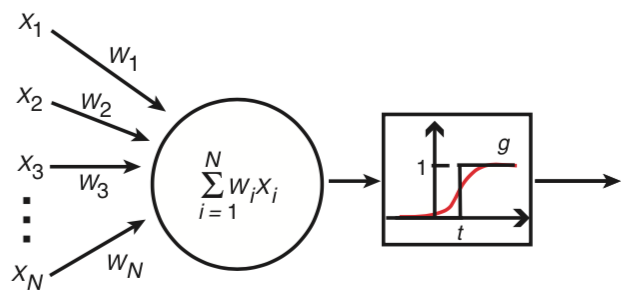
\includegraphics[width=0.5\linewidth]{graphics/krogh/krogh_neural-network.png}
    \caption*{Quelle: \textcite{Krogh2008}}
%\end{wrapfigure}
\end{figure}

Damit ein Neuronales Netzwerk Leistungsfähig werden kann, muss es ähnlich wie ein Mensch, erst lernen. Für das Neuronale Netzwerk bedeutet Lernen, für die Gewichte und den Threshod geeignete Werte zu finden. Dieses computersimulierte Lernen, auch Machine Learning genannt, funktioniert dabei so, dass für die Gewichte der Verbindungen, sprich die stärke der Synpasen, ein zufälliger Wert gewählt wird. Anschliessend wird eine Übungsaufgabe vom Netzwerk gelöst. Das Resultat des Netzwerks ist zu Beginn höchstwahrscheinlich falsch und die Gewichte im Netzwerk werden mit einem kleinen Schritt angepasst. Es werden dann immer weitere Aufgaben gelöst und die Gewichte entsprechend angepasst bis das Netzwerk die gewünschten Resultate liefert~\autocite{Krogh2008}.
Dieses Training kann durch verschiedene Algorithmen implementiert werden. Einer davon wird im Kapitel \ref{chap:backpropagation} beschrieben.

Seit mehreren Jahren liefern Neuronale Netzwerke bessere Resultate als klassische Techniken. Dabei werden Neuronale Netzwerk vorwiegend für visuelle Aufgaben und immer häufiger auch zur Verarbeitung Natürlicher Sprache verwendet~\autocite{Olah2014b}.

% \todo[inline]{Say a word on overfitting}

% \todo[inline]{Say something about learning strategies (supervised / unsupervised)}

\subsection{Tiefe Neuronale Netzwerke}

Neuronale Netzwerke finden oft bei Klassifizierungsproblemen Anwendung. Dabei soll aufgrund bestimmter Eingabewerte eine Klasse bestimmt werden. Ein Beispiel dafür ist die Klassifizierung eines Säugetiers in die Klasse Hund oder Katze aufgrund ihrer Merkmale~\autocite{Krogh2008}.

Einfache Netzwerke von Threshold Units können Klassifizierungsprobleme dann Lösen, wenn die Klassen linear separierbar sind. Die Abbildung \ref{krogh:b} veranschaulicht die lineare Separierung mit Hilfe einer Ebene in einem dreidimensionalen Raum. Die Ebene separiert die grünen und roten Punkte voneinander~\autocite{Krogh2008}.

%\begin{wrapfigure}{l}{0.4\textwidth} 
\begin{figure}[h]
    \captionsetup{width=.9\linewidth}
    \caption{Die graue Ebene zeit das Konzept der linearen Separierbarkeit. Die grünen und roten Punkte können durch eine lineare Ebene separiert werden. Die grünen und roten Kreuze liegen allerdings auf der falschen Seite der Ebene. Aufgrund dieser Kreuze ist die abgebildete Problemstellung nicht linear separierbar.}
    \label{krogh:b}
    \centering
    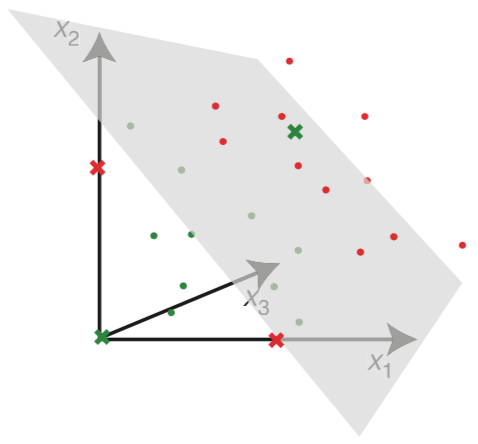
\includegraphics[width=0.4\linewidth]{graphics/krogh/krogh_plane.png}
    \caption*{Quelle: \textcite{Krogh2008}}
%\end{wrapfigure}
\end{figure}

Der Abbildung \ref{krogh:b} ist zu entnehmen, dass die Problemstellung im abgebildeten Fall, wie die meisten Klassifizierungsprobleme, nicht linear separierbar ist. Die roten und grünen Kreuze markieren dabei Punkte, welche auf der falschen Seite der Ebene liegen. Eine Klassifizierung durch ein einfaches Netzwerk von Threshold Units würde die Klasse dieser Datensätze falsch vorhersagen~\autocite{Krogh2008}.

Um das Modell zur Klassifizierung zu verbessern, können weitere Ebenen in den dreidimensionalen Raum eingesetzt werden. Durch eine weitere Ebene ist es dem Modell möglich, mehr Datensätze richtig zu klassifizieren. Neue Ebenen werden mit neuen Schichten von Threshold Units modelliert (vgl. Abbildung \ref{krogh:c}). Diese neuen Schichten, welche zwischen die Eingabe und Ausgabe Schichten platziert werden, werden Versteckte Schichten (Hidden Layers) genannt~\autocite{Krogh2008}.

% \begin{wrapfigure}{l}{0.4\textwidth} 
\begin{figure}[h]
    \captionsetup{width=.9\linewidth}
    \caption{Modell eines tiefen neuronalen Netzwerk mit einer versteckten Schicht (Hidden Layer).}
    \label{krogh:c}
    \centering
    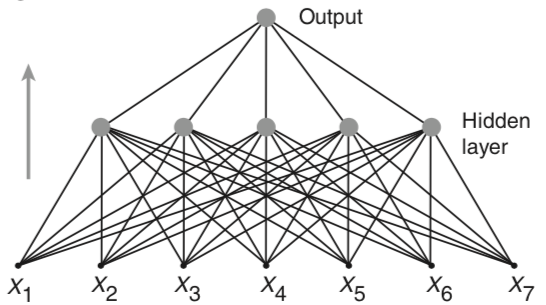
\includegraphics[width=0.4\linewidth]{graphics/krogh/krogh_deep-network.png}
    \caption*{Quelle: \textcite{Krogh2008}}
%\end{wrapfigure}
\end{figure}

Ein Netzwerk mit mehreren Schichten, auch tiefes neuronales Netzwerk (Deep Neural Network) genannt, stellt aber neue Anforderungen an das Training. Ein Netzwerk mit versteckten Schichten kann nicht mehr auf eine analytische Weise trainiert werden. Aus diesem Grund wird ein komplexerer Lernalgorithmus benötigt. Ein solcher Algorithmus wird im nächsten Kapitel beschrieben~\autocite{Krogh2008}. 

\todo[inline]{\textcite{MLYearning} chapter 4: scale drives machine learning progress}

\subsection{Backpropagation}
\label{chap:backpropagation}

Da, wie bereits im vorherigen Kapitel erwähnt, tiefe neuronale Netzwerke zu Komplex sind, um mit einem analytischen Ansatz trainiert zu werden, muss ein anderes Vorgehen gefunden werden. Das meist verwendetste Vorgehen zum Training von tiefen neuronalen Netzwerken ist das sogenannte Backpropagation. Beim Backpropagation werden erst zufällige Gewichte und Thresholds festgesetzt. Das Netzwerk löst mit diesen zufälligen Gewichten und Thresholds eine erste Übungsaufgabe. Die Abweichung vom erwarteten Resultat (der sogenannte Fehler) wird nun quadriert. Ziel des Backpropagation ist es nun, diesen quadrierten Fehler zu minimieren. Dies wird gemacht, indem das Verfahren des steilsten Abstiegs, auch Gradientverfahren (englisch gradient descent), angewendet wird. Mit Hilfe dieses Verfahrens zur Lösung allgemeiner Optimierungsprobleme aus der Numerik werden nun die Gewichte und der Threshold so angepasst, dass der quadrierte Fehler minimiert wird. Dieses Vorgehen wird nun mit weiteren Übungsaufgaben wiederholt, bis sich der quadrierte Fehler nicht mehr verändert~\autocite{Krogh2008}.

Beim Backpropagation müssen einige Probleme beachtet werden. So kann durch das Gradientverfahren nur ein lokales Minimum gefunden werden. Ob dieses lokale Minimum dem globalen Minimum entspricht, ist nicht bekannt. Das Ergebnis des Trainings ist also stark von den zufällig gewählten Startwerten der Gewichte und Thresholds abhängig~\autocite{Krogh2008}.

Die grösste Problematik beim Trainieren von neuronalen Netzwerken, besonders von tiefen neuronalen Netzwerken, ist die Gefahr des sogenannten Overfitting oder Auswendiglernen~\autocite{Krogh2008}. Diese Problematik wird im folgenden Kapitel genauer erläutert.

\subsection{Overfitting}

\todo[inline]{Extend this paragraph with some words about Underfitting and the views from the deeplearning.ai book (see iBooks)}

Das sogenannte Overfitting, oder auch Auswendiglernen, bezeichnet die Problematik, dass sich ein Modell aufgrund zuvieler Parameter bei zu wenig Trainingsdaten zu stark an die Trainingsdaten anpasst. Das Modell kann die Trainingsdaten mit 100\% Treffergenauigkeit Beurteilen. Soll das Modell dann aber einen neuen Datensatz beurteilen, so sinkt die Treffergenauigkeit massiv~\autocite{Krogh2008}.

% \begin{wrapfigure}{l}{0.4\textwidth} 
\begin{figure}[h]
    \caption{Overfitting... TODO}
    \label{krogh:d}
    \centering
    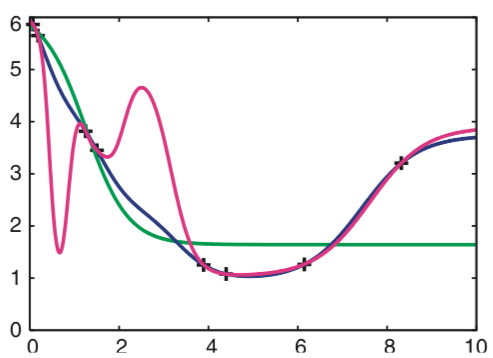
\includegraphics[width=0.4\linewidth]{graphics/krogh/krogh_overfitting.png}
    \caption*{Quelle: \textcite{Krogh2008}}
%\end{wrapfigure}
\end{figure}

Die Problematik des Overfitting ist aus der Mathematik bekannt. Hat eine Funktion zu viele freie Parameter, so passt sie sich zu stark an die vorgegebenen Punkte an. Abbildung \ref{krogh:d} veranschaulicht diese Problematik. Die grüne Funktion liefert kein optimales Ergebnis, da zu wenige Parameter vorhanden sind. Die pinke Funktion hat dagegen zuviele Parameter und lernt die Trainingsdaten perfekt. Um dies zu erreichen ist die pinke Funktion aber etwas sehr kreativ in ihren Wendepunkten. Die blaue Funktion bietet ein gesundes Mittelmass~\autocite{Krogh2008}.

Während die Problematik des Overfitting aus anderen Bereichen bereits bekannt ist, scheinen neuronale Netzwerke besonders anfällig für eine solche überparametrierung. Würden wir ein Modell entwickeln, welches anhand 20 Merkmalen (20 Eingabewerte) mit Hilfe einer verstecken Schicht von 10 Neuronen erkennen soll, ob es sich um einen Hund oder eine Katze handelt, so würden 221 Parameter geschaffen. Jeder der 20 Eingabewerte wird durch ein Gewicht mit den 10 Neuronen aus der versteckten Schicht Verbunden ($10 * 20 = 200$ Parameter). Jedes dieser Neuronen hat einen Threshold (10 Parameter) und ist mit dem Ausgabeneuron verknüpft (10 Parameter). Das Ausgabeneuron selbst hat auch wieder einen Threshold (1 Parameter). Wird dieses Modell mit 221 Parametern nun mit Hilfe von nur 100 Trainingsdatensätzen trainiert, so kann es diese problemlos Auswendig lernen~\autocite{Krogh2008}.

Um ein solches Overfitting zu verhindert stehen diverse Techniken zur Verfügung. Eine beliebte Regularisierungstechnik ist es, eine sogenannte Dropout Schicht in das Netzwerk einzubringen. Diese Dropout Schichte deaktiviert während dem Training zufällige Neuronen\todo{Mehr zu Dropout, Quelle zu Dropout}~\autocite{Krogh2008, TODO_Dropout}.  

Um ein Overfitting zu erkennen, ist es wichtig, ein neuronales Netzwerk an Daten zu testen, welche nicht zum Training verwendet werden~\autocite{Krogh2008}. \todo{Etwas mehr zum erkennen von Overfitting. Steigendes validation loss, sinkde validation accuracy, Validation accuracy ist stets < training accuracy}

\subsection{Long-Short-Term-Memory Netzwerke}

Menschen starten ihren Denkprozess nicht jede Sekunde von neuem. Beim Lesen wird jedes Wort aufgrund des Verständnisses des vorherigen Wortes verstanden. Gedanken sind persistent. Genau solche persistenten Gedanken sind mit dem bisherigen Ansätzen für Neuronale Netze nicht modellierbar. Hier kommen Recurrent Neural Networks (kurz RNN) ins Spiel. Recurrent Neural Networks sind Neuronale Netzwerke mit integrierten Schlaufen~\autocite{Olah2015}. 

In Abbildung \ref{rnn1} wird ein RNN mit einer Schlaufe dargestellt. Daneben ist das selbe Netzwerk in einer anderen, ausgerollten Weise zu sehen. Die Abbildung verdeutlicht, wie Informationen von einem Neuron zum anderen fliessen können. Mit diesem Informationsfluss von Neuron zu Neuron werden die Resultate jeweils von den vorhergehenden Neuronen beeinflusst. Damit wird eine Art Kurzzeitgedächtnis geschaffen, welches dem Neuronalen Netzwerk erlaubt mit Kontextinformationen zu arbeiten~\autocite{Olah2015}.
\begin{figure}[h]
    \captionsetup{width=.8\linewidth}
    \caption{Infromationsfluss durch ein Recurrent Neural Network dargestellt als Schlaufe (links) und als Sequenz (rechts)}
    \label{rnn1}
    \centering
    \vspace{0.2cm}
    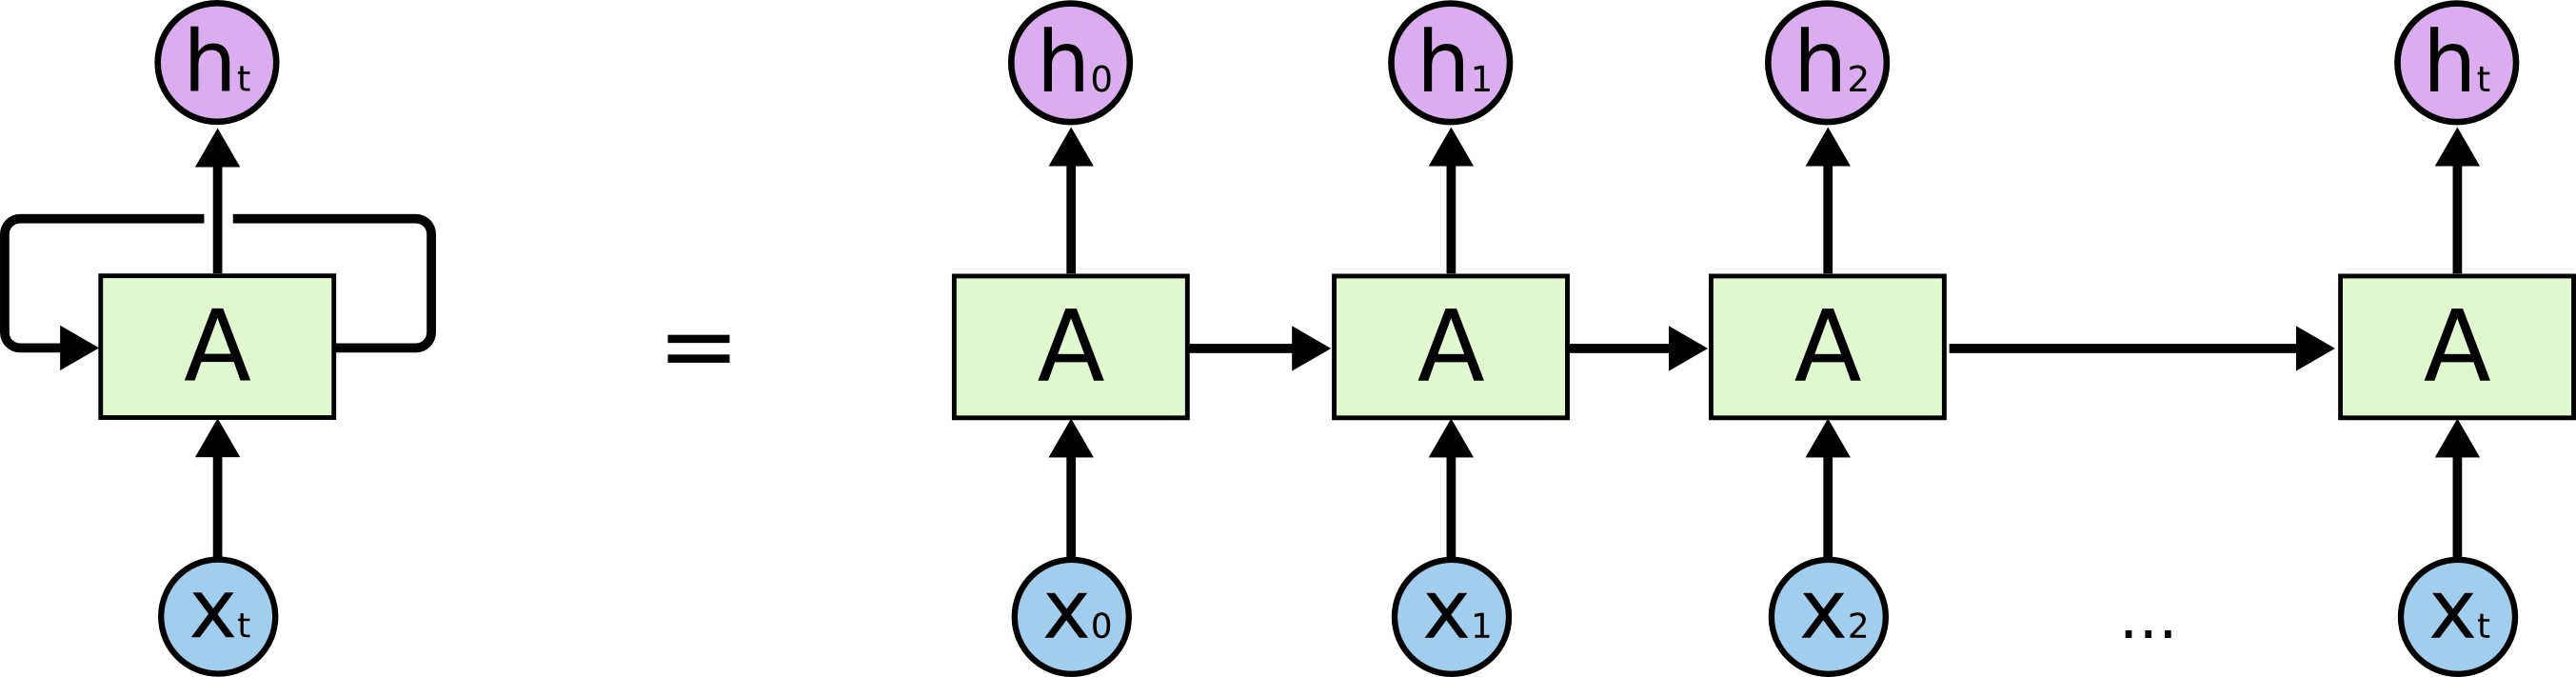
\includegraphics[width=0.6\textwidth]{graphics/rnn1.png}\\
    \vspace{0.3cm}
    \caption*{Quelle: \textcite{Olah2015}}
\end{figure}

Ein Problem von RNNs ist, dass nur ein Kurzzeitgedächtnis zur Verfügung steht. Liegen Informationen etwas länger zurück, sprich der Abstand zwischen den beiden relevanten Neuronen ist zu gross, gehen diese Informationen verloren. Eine Lösung für diese Problematik bieten Long-Short-Term-Memory (kurz LSTM) Netzwerke. Diese Spezialform von Recurrent Neural Networks arbeitet mit sogenannten Gates, um zu regulieren, wie viel Kontextinformationen behalten oder vergessen werden sollen. Mit vier solchen Gates, bestehend aus einem Neural Network Layer und einer Pointwise Operation (vgl. Abbilung \ref{lstm1}), ist ein LSTM Netzwerk in der Lage, nicht nur ein Kurz- sondern auch ein Langzeitgedächtnis aufzubauen~\autocite{Olah2015}.
\begin{figure}[h]
    \captionsetup{width=.8\linewidth}
    \caption{Veranschaulichung des Informationsflusses eines LSTM Netzwerk mit seinen vier internen Schichten}
    \label{lstm1}
    \centering
    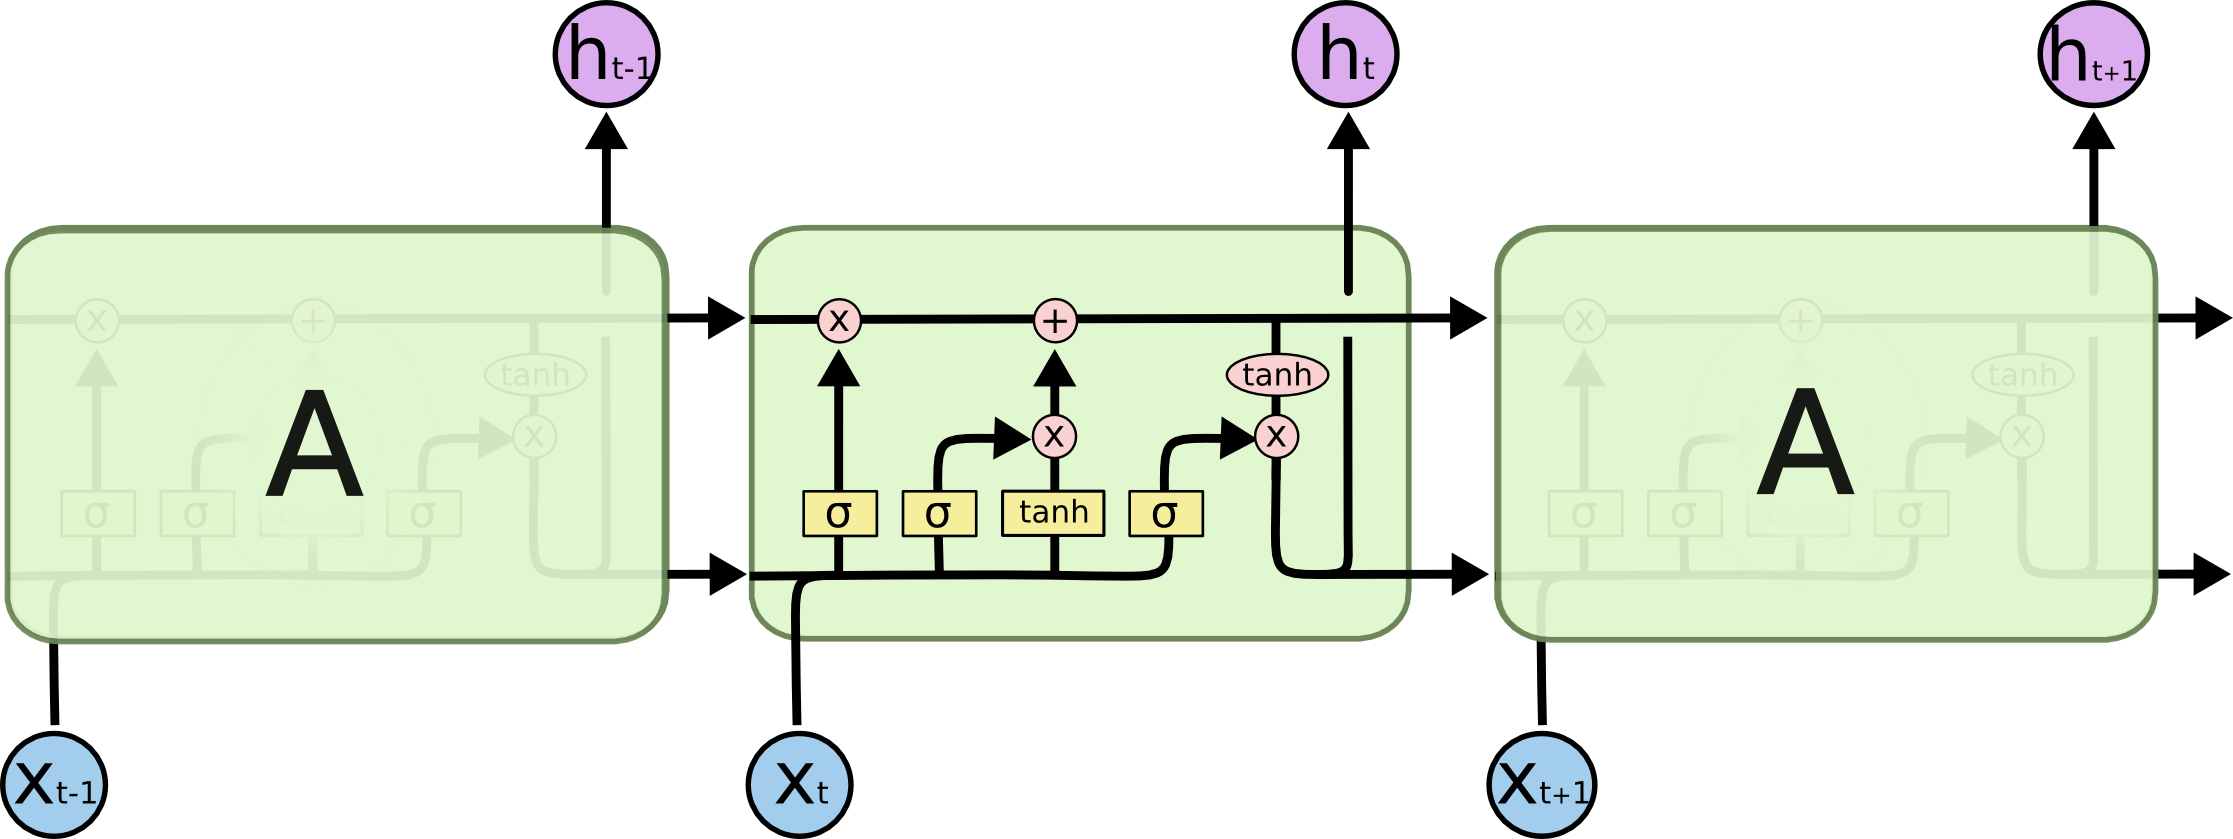
\includegraphics[width=0.6\textwidth]{graphics/lstm.png}\\
    \vspace{0.5cm}
    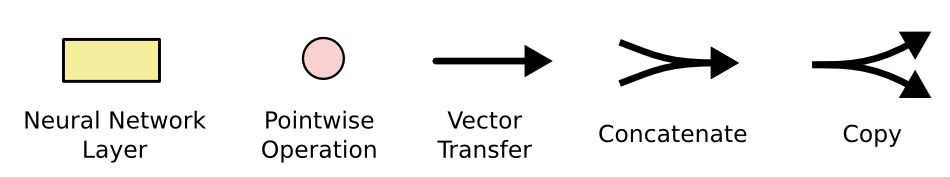
\includegraphics[width=0.6\textwidth]{graphics/lstm-notation.png}\\
    \vspace{0.1cm}
    \caption*{Quelle: \textcite{Olah2015}}
\end{figure}

Recurrent Neural Networks wurden in der Vergangenheit sehr erfolgreich für viele Aufgaben, wie beispielsweise die Spracherkennung, Sprachmodellierung, maschinelle Übersetzung sowie Bilderkennung, angewendet. In den meisten Fällen wurden dabei LSTM Netzwerke angewendet, da die Resultate um ein Vielfaches besser ausfallen als mit herkömmlichen RNNs~\autocite{Olah2015}.

LSTM Netzwerke sind für diese Arbeit besonders zur Texterkennung und Rechtschreibkorrektur interessant. Diese beiden Techniken werden im Prototypen der Rechnungsindexierung verwendet.

\subsection{Texterkennung}

Ein wichtiger Bestandteil des Prototypen zur Indexierung von Rechnungen ist die Erkennung von Texten, ob Druckbuchstaben oder Handschrift, auf den Rechnungen. Die erkannten Texte bilden die Grundlage für jegliche digitale Verarbeitung der Rechnungen.

Die herkömmliche Feature-detection in Texterkennungssoftware wird immer mehr mit künstlicher Intelligenz ersetzt. \textcite{Neuberg2017} beschreibt wie Dropbox künstliche Intelligenz anwendet, um Texte aus Fotografien von Dokumenten durchsuchbar zu machen. Zur Anwendung kommen dabei verschiedene Techniken aus dem Bereich der künstlichen Intelligenz: \textit{Convolutional Neural Network}\footnote{Ein Convolutional Neural Network ist eine Spezialform eines Neuronalen Netzwerks bei welchen, etwas vereinfacht ausgedrückt, viele Kopien des gleichen Neurons zum Einsatz kommen\autocite{Olah2014}.} (CNNs),  \textit{Long-Short-Term-Memory} (LSTM) Netzwerke, \textit{Connectionist Temporal Classification}\footnote{CTC ist ein Konzept aus dem Training von Neuronalen Netzwerken, welches vor allem in der Handschrifterkennung Verwendung findet. Dabei wird eine spezielle Trainingsfunktion verwendet, durch welche die Positionierung von Buchstaben generalisiert und somit der Lernprozess des Neuronalen Netzwerks vereinfacht werden kann~\autocite{Scheidl2018}} (CTC) und weitere~\autocite{Neuberg2017}.

Auch die Texterkennungssoftware Tesseract, welche ursprünglich als PhD Forschungsprojekt im HP Lab entwickelt wurde und seit 2005 als Open Source Software zur freien Verfügung steht, verwendet seit Version 4 künstliche Intelligenz~\autocite{Smith2007}. So wurde die Feature-detecion durch ein LSTM Netzwerk mit mehr als 100 Schichten ersetzt. Die Texterkennung konnte so nicht nur Qualitativ stark verbessert werden sondern ist auch einiges schneller als zuvor. Doch auch nach den Verbesserungen sind die Ergebnisse nicht perfekt und müssen fallspezifisch optimiert werden~\autocite{O.V.2018, O.V.2018a}.

\subsection{Word embedding}

Neuronale Netzwerke funktionieren mit Zahlen. Damit auch Wörter und ganze Sätze von solchen Netzwerken verarbeitet werden können, muss eine geeignete Repräsentation von Wörtern durch Zahlen gefunden werden. Der Prozess, mit welchem ein Wort in eine zahlen-basierte Repräsentation gebracht wird, nennt sicht Word embedding~\autocite{Olah2014b}.

Die ersten Word embeddings wurden von \textcite{Bengio2001} eingeführt. Trotz des schon fortgeschrittenen Alter dieses Forschungsgebiet ist es noch immer hoch interessant und in voller Fahrt~\autocite{Olah2014b}.

\begin{wrapfigure}{r}{0.5\textwidth} 
    \caption{Modulares Netzwerk zur Validierung von 5-Grammen mit einer Word embedding Funktion ($W$) und einem Neuronalen Netzwerk ($R$)}
    \label{wordembeddingtraining}
    \centering
    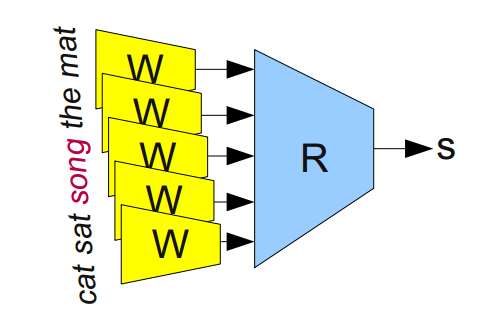
\includegraphics[width=0.48\textwidth]{graphics/wordembeddingtraining.png}
    \caption*{Quelle: \textcite{Olah2014b}}
\end{wrapfigure}
Technisch gesehen ist ein Word embedding eine parametrierte Funktion, welche Wörter einer bestimmten Sprache in einen hoch-dimensionalen Vektor (typischerweise 200-500 Dimensionen) transformiert. Um diese hoch komplexe Funktion zu definieren, kommt, wie bei den Neuronalen Netzwerken, Machine Learning zum Einsatz. \textcite{Olah2014b} beschreibt in seinem Artikel ein Beispiel, bei welchem eine solche Word embedding Funktion trainiert wird, indem die Resultate aus dem Word embedding in ein Neuronales Netzwerk zur Prüfung eines 5-Grammes gespiesen werden und dann das Gesamtkonstrukt trainiert wird (vgl. Abbildung \ref{wordembeddingtraining})~\autocite{Olah2014b}.

Um sich Word embeddings besser vorstellen zu können, zieht \textcite{Olah2014b} zwei verschiedene Möglichkeiten der Visualisierung heran.

Die erste Visualisierung bedient sich dem t-SNE Algorithmus um die hoch-dimensionalen Vektoren in einem zweidimensionalen Diagramm darzustellen. In diesem Diagramm ist klar zu erkennen, dass ähnliche Wörter nahe zusammen sind (vgl. Abbildung \ref{wordembeddingtsne})~\autocite{Olah2014b}.
\begin{figure}[h]
    \centering
    \caption{t-SNE Darstellung eines Word embeddings, die verdeutlicht, dass ähnliche Wörter ähnliche Vekotren aufweisen}
    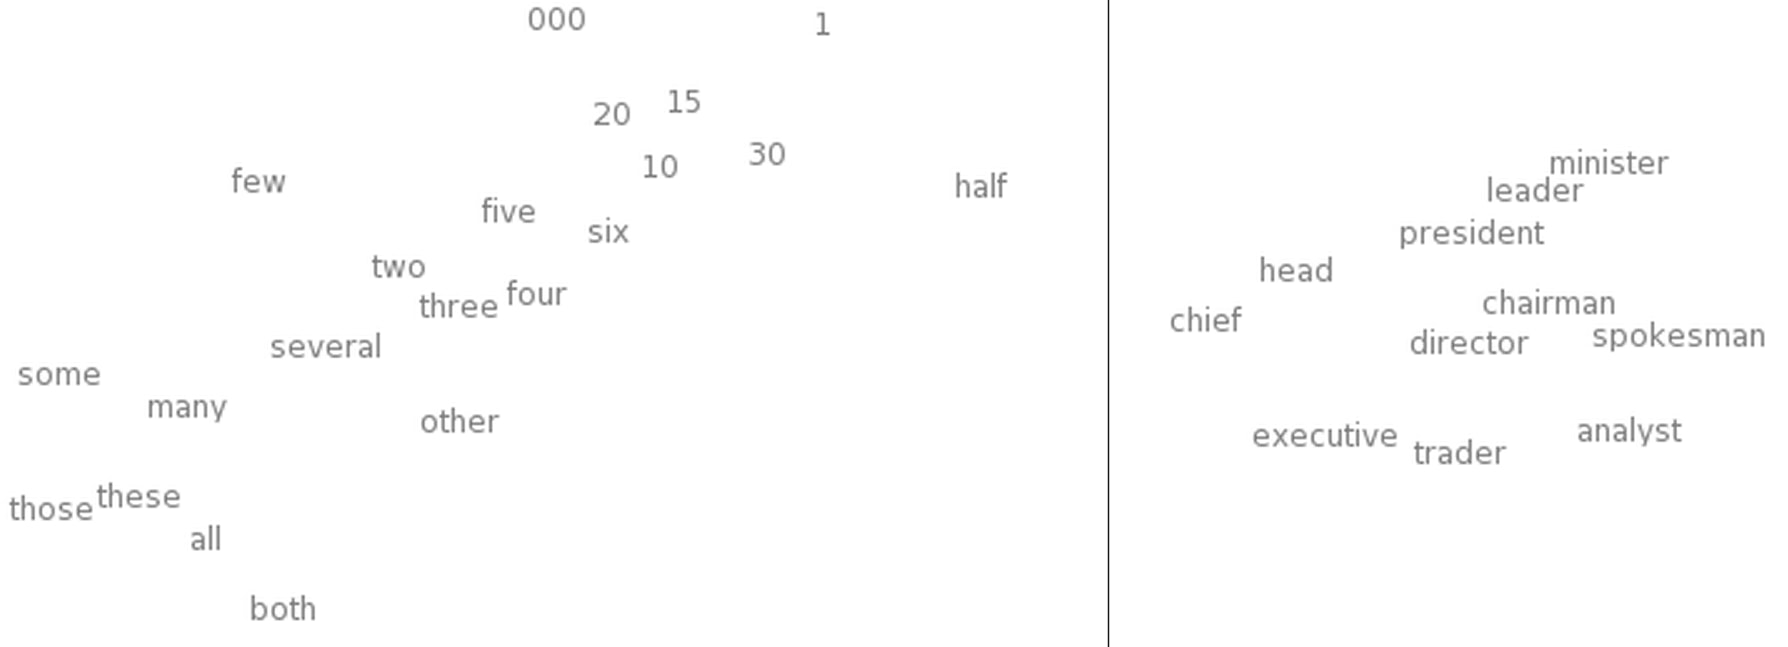
\includegraphics[width=\textwidth]{graphics/wordmebeddingtsne.jpg}
    \caption*{Quelle: \textcite{Turian2010} in \textcite{Olah2014b}}
    \label{wordembeddingtsne}
\end{figure}

Die zweite Visualisierung listet in einer Tabelle (vgl. Tabelle \ref{wordembeddingtable}) für sechs Wörter die nächsten Embeddings, sprich mit den mathematisch nächsten Vektoren, auf. So werden beispielsweise unter dem Titel \textit{FRANCE} neben \textit{EUROPA} diverse weitere Länder aufgelistet.
\begin{table}[h]
\centering
    \caption{Sechs Ausgangswörter mit den ihnen ähnlichsten Word embeddings, sprich mit den mathematisch nächsten Vektoren}
    \label{wordembeddingtable}
    \renewcommand{\arraystretch}{1.25}
    \setlength{\tabcolsep}{3pt}
    \small
    \begin{tabular}{ | l | l | l | l | l | l |}
    \hline
    \rowcolor{ccc} FRANCE & JESUS & XBOX & REDDISH & SCRATCHED & MEGABITS \\ \hline
    AUSTRIA & GOD & AMIGA & GREENISH & NAILED & OCTETS \\ \hline
    BELGIUM & SATI & PLAYSTATION & BLUISH & SMASHED & MB/S \\ \hline
    GERMNAY& CHRIST & MSX & PINKISH & PUNCHED & BIT/S \\ \hline
    ITALY & SATAN & IPOD & PRUPLISH & POPPED & BAUD \\ \hline
    GREECE & KALI & SEGA & BROWNISH & CRIMPED & CARATS \\ \hline
    SWEDEN & INDRA & PS\textit{NUMBER} & GREYISH & SCRAPED & KBIT/S \\ \hline
    NORWAY & VISHNU & HD & GRAYISH & SCREWED & MEGAHERTZ \\ \hline
    EUROPE & ANANDA & DRAMCAST & WHITISH & SECTIONED & MEGAPIXELS \\ \hline
    HUNGARY & PARVATI & GEFORCE & SILVERY & SLASHED & GBIT/S \\ \hline
    SWITZERLAND & GRACE & CAPCOM & YELLOWISH & RIPPED & AMPERES \\ \hline
    \end{tabular}
    \caption*{Quelle: \textcite{Collobert2011} in \textcite{Olah2014b}}
\end{table}

Sowohl Abbildung \ref{wordembeddingtsne} als auch Tabelle \ref{wordembeddingtable}, zeigen die Stärke von Word embeddings auf: Ähnliche Wörter werden mit ähnlichen Vektoren versehen und so wird eine komplexe Landschaft von Zusammengehörigen Wörtern gebildet. Aufgrund dieser Eigenschaft verändert sich durch den Austausch eines Wortes mit einem Synonym der Input-Vektor für ein nachfolgendes Neuronales Netzwerk nur geringfügig, da die Word embeddings der beiden Synonyme sehr ähnlich sind. Somit muss dieses nachfolgende Neuronale Netzwerk nicht für alle Wörter der Welt trainiert werden, sondern kann auf die Generalisierung durch das Word embedding aufbauen~\autocite{Olah2014b}.

Word embeddings sind zu einem extrem wichtigen Baustein bei der Verarbeitung von Natürlichen Texten geworden. Neben Input und Output Repräsentationen bei NLP Tasks können Word embeddings auch Output Repräsentationen in der Bilderkennung sein~\autocite{Olah2014b}. 

Für den Prototypen bilden Word embeddings eine wichtige Grundlage, da durch diese Technik die in den Rechnungen enthaltenen Wröter und Sätze in eine generalisierte, durch Neuronale Netzwerke verarbeitbare Form gebracht werden können.

\subsection{Korrektur von Rechtschreibung und Grammatik}

Trotz grossem Fortschritt, nicht zuletzt dank der Verwendung von künstlicher Intelligenz, im Bereich der Texterkennung, werden Texte nicht zu 100\% korrekt erkannt. So schleichen sich falsch erkannte Buchstaben ein, welche nicht nur Wörter sondern auch ganze Sätze bedeutungslos machen. Um solche Fehler zu korrigieren, wird auf die Rechtschreibung- und Grammatik-Korrektur zurückgegriffen. Während diverse Korrekturprogramme regelbasierte Software anwenden, wurde auch in diesem Bereich bereits erfolgreich künstliche Intelligenz angewandt.

Mit Hilfe der in einem vorherigen Kapiteln eingeführten Technik des Word embeddings und von LSTM Netzwerken lässt sich diese Problematik angehen. So kann ein Modulares Netzwerk aus Word embeddings und mehreren LSTM Schichten verwendet werden, um eine Rechtschreibkorrektur vorzunehmen. So beschreibt \textcite{Weiss2016} in seinem Blog, wie mit einem einfachen Neuronalen Netzwerk, bestehend aus nur 4 LSTM und 4 Dropout Schichten, bereits erfolgreich Rechtschreibfehler korrigiert werden können. 

% can't use wrapfigure here as otherwise the next sections wraps too
\begin{figure} % wrapfigure}{l}{0.5\textwidth}
    \centering
    \caption{Vergleich der Erfolgsrate bei der Prüfung von 418 Textsnippets}
    \label{deepgrammar}
    \begin{tikzpicture}
        \begin{axis}[
            ytick={0,10,20,30,40,50,60,70},
            ymin=0,
            ymax=70,
            xticklabels=\empty,
            xtick style={draw=none},
        	ylabel={Erfolgsrate [\%]},
        	enlargelimits=0.05,
        	ybar={10pt},
            bar width=20pt,
            legend style={cells={anchor=west},at={(1,-0.02)}, legend columns=2}, 
            area legend,
        ]
            \addplot[fill=cChart1]
            	coordinates {(0,61)};
            \addplot[fill=cChart2]
            	coordinates {(0,54)};
            \addplot[fill=cChart3]
            	coordinates {(0,54)};
            \addplot[fill=cChart4]
            	coordinates {(0,65)};
            \addplot[fill=cChart5]
            	coordinates {(0, 58)};
            \legend{Word,Grammarly,Google,LanguageTool,Deepgrammar}
        \end{axis}
    \end{tikzpicture}
    \caption*{Quelle: In Anlehnung an \textcite{Mugan}}
\end{figure} %wrapfigure}
Nicht nur zur Korrektur von Rechtschreibfehler ist ein Neuronales Netzwerk anwendbar. So kann unter deepgrammar.com ein Experiment gefunden werden, bei welchem ein solches Netzwerk zur Grammatikprüfung angewendet wird. Die Resultate, welche in der Tabelle \ref{deepgrammar} zu sehen sind, sind erstaunlich. Obwohl DeepGrammar erst seit einem Jahr existiert und dabei von nur einer Person entwickelt wurde, funktioniert das Netzwerk beinahe so gut wie \textit{Microsoft Word}\footnote{Microsoft Word ist ein Programm zur Textverarbeitung und Dokumenterstellung von Microsoft~\autocite{MicrosoftCorporation2018}.} oder \textit{Language Tool 3.1}\footnote{\enquote{LanguageTool ist eine Software zur Textprüfung [...]}~\autocite{LanguageTool2018}} und sogar besser als \textit{Grammarly}\footnote{Grammarly verspricht präzise, kontextabhängige Korrekturen von Texten~\autocite{GramarlyInc.2018}} und \textit{Google Docs}\footnote{Google Docs ist eine Online-Lösung zur Textverarbeitung von Google~\autocite{GoogleLLC2018}}~\autocite{Mugan}.

% TODO: Mugan erwähnt eine bessere Studie. In der Thesis diese verwenden, da Zahlen aus DeepGrammar nicht 100% korrekt sind https://arxiv.org/pdf/1807.01270.pdf

Ein weiterer grosser Vorteil von Neuronalen Netzwerken zur Fehlerkorrektur erwähnt \textcite{Mugan2018} in einer persönlichen Kommunikation: Das Neuronale Netzwerk kann auf das Domänenspezifische Lexikon trainiert werden. Das Netzwerk kann beispielsweise mit medizinischen Begriffen aus den Rechnungen trainiert werden, so dass die Resultate des in dieser Arbeit entwickelten Prototypen noch besser werden~\autocite{Mugan2018}.

\subsection{Informationsextraktion aus natürlichen Texten}

% https://en.wikipedia.org/wiki/Named-entity_recognition
% https://en.wikipedia.org/wiki/Medical_classification

Informationsextraktion beschreibt das Themengebiet rund um die Extraktion von strukturierten Informationen aus unstrukturiertem oder halb-strukturiertem Text. In diesem Kapitel werden einige Techniken aus diesem Themengebiet kurz erläutert und deren Ein\-satz\-mög\-lich\-keit für die Entwicklung des Prototypen diskutiert.

Eine \textit{Regular Expression} (kurz RegEx) ist ein Ausdruck, welcher eine Zeichenkette beschreibt. Diese Ausdrücke funktionieren ähnlich wie arithmetische Ausdrücke: Es werden Operatoren verwendet, um mehrere Ausdrücke zu einem komplexeren Ausdruck zusammenzufassen\autocite{Xiao2004}.

\textcite{Xiao2004} beschreibt als einfaches Beispiel den Ausdruck \texttt{[a,p]m [0-9]+:[0-9]+} um Zeitangaben wie AM 12:45 zu extrahieren. Dieses Beispiel zeigt einerseits die Einfachheit dieser Technik aber auch die Grenzen. 12:45 AM wird beispielsweise nicht erkannt, da AM hier nach anstelle vor der Uhrzeit steht. 

Ein weiterer Nachteil von Regular Expressions ist, dass Kontextinformationen nicht be\-rück\-sich\-tigt werden. Folgendes Beispiel von \textcite{Xiao2004} zeigt dies auf: Der Ausdruck \texttt{[0-9]+} ist zwar in der Lage aus dem Text \texttt{100\$} die Zahl \texttt{100} zu extrahieren, allerdings geht die Information, dass es sich hier um einen Geldbetrag handelt, verloren.

Um eine hohe Präzision bei der Informationsextraktion zu ermöglichen, sollten Regular Expressions also nur mit Vorsicht und in Kombination mit anderen Techniken verwendet werden~\autocite{Xiao2004};

Trotz der Nachteile der Regular Expressions können diese in der Entwicklung des Prototypen hilfreich sein. In Rechnungen werden viele Beträge, Daten und ähnliche Ausdrücke verwendet, welche mit Regular Expressions erkannt werden können.

\textit{Named Entity Recognition and Classification} (kurz NERC oder NER), beschreibt das erkennen und kategorisieren von Entitäten, sprich Wörter oder Wortgruppen aus natürlichen Texten~\autocite{Nadeau2007}.

Der Begriff \textit{Named Entity} wurde bei der Formulierung der Aufgabenstellung der sechsten Message Understanding Conference im Jahre 1995 definiert~\autocite{Borthwick1998}. So wurde bereits damals erkannt, dass die Extraktion von Namen, von Personen, Organisationen oder Lokationen, nummerischen Ausdrücken, Daten und Prozent-Ausdrücken wichtig ist~\autocite{Nadeau2007}.

Für die Named Entity Recognition and Classification stehen einige freie Softwarelösungen zur Verfügung. So veröffentlicht beispielsweise Stanford eine Java Implementierung und SpaCy, eine Sammlung von Natural Language Processing Software, beinhaltet eine Implementierung in Python~\autocite{StanfordNLPGroup, ExplosionAI}.

Die Anwendung von NERC ist für das Fallbeispiel äusserst Interessant. Die Erkennung von Namen von Personen ist hilfreich zur Erkennung des Patienten und des Leistungserbringers. Weiter hilft die Erkennung von Daten der Ermittlung des Behandlungsdatums und nicht zuletzt kann durch die Erkennung und Klassifizierung von nummerischen Ausdrücken der Gesamtbetrag sowie die Beträge einzelner Positionen ermittelt werden.

Die letzte Technik welche in diesem Kapitel erläutert wird, ist das \textit{Part of Speech Tagging} (kurz PoS-Tagging). Beim PoS-Tagging werden Wörter und Satzzeichen ihren Wortarten (Nomen, Adjektive, etc.) zugewiesen~\autocite{Xiao2004}.

Die grösste Herausforderung beim PoS-Tagging sind Wörter welche verschiedenen Wortgruppen zugewiesen werden könnten. Beispielsweise kann das Wort \textit{widerwillig} im Satz \textit{Sie nannten den Täter widerwillig.} als Adjektiv oder Adverb aufgefasst werden und somit die Bedeutung des Satzes vollkommen verändern~\autocite{Volk}.

% Es gibt diverse Arten von Implementierung des PoS-Tagging, welche in regelbasierte, stochastische und neuronale Verfahren unterteilt werden können. Ein weit verbreiteter Ansatz ist die Verwendung von Hidden Markov Modellen. Ein Hidden Markov Modell ist ein stochastisches Modell, welches Zustände mit übergangswahrscheinlichkeiten modelliert.

Die Verwendung von PoS-Tagging kann bei Rechnungen mit einem Prosatext von Vorteil sein. Wie viele relevante Informationen in Prosatexten von Rechnungen verborgen sind, muss sich aber erst noch zeigen.

Die beschriebenen Techniken bieten eine gute Grundlage um damit eine erste Implementierung eines Prototypen zur Rechnungsindexierung zu beginnen.

\subsection{Bewertung eines KI Systems}

Um ein System objektiv zu Bewerten und mit anderen Ansätzen zu vergleichen, bedarf es Metriken. Folgend werden einige Metriken erläutert und ihre Anwendungsfälle diskutiert.

\subsubsection{Treffergenauigkeit}

Die Treffergenauigkeit, englisch Accuracy (kurz acc), ist die Metrik, welche wohl am meisten im Zusammenhang mit der künstlichen Intelligenz zu finden ist. Die Frage ist aber, ob diese Metrik für alle Anwendungsfälle geeignet ist~\autocite{TDSAccuracy}.

Die Treffergenauigkeit sagt aus, wie viele der Vorhersagen eines Systems der Wirklichkeit entsprechen. Die Formell lautet wie folgt~\autocite{TDSAccuracy}: 

$$Accuracy = 1 - \frac{False Positive + False Negative}{Total Records}$$

Die Confusion Matrix in Abbildung \ref{cm-sample} zeigt ein Beispiel mit einer Treffergenauigkeit von 0.99, respeketive 99.9\%. Aus 1000 Datensätzen wurden 998 korrekt als Negativ klassifiziert. Ein Datensatz wurde korrekt als Positiv klassifiziert und ein Datensatz wurde fälschlicherweise als Negativ klassifiziert~\autocite{TDSAccuracy}.

\begin{figure}[h]
    \centering
    \def\arraystretch{1.5}
    \arrayrulecolor{black}
    \begin{tabular}{llcc}
        \multicolumn{2}{l}{}                                                                       & \multicolumn{2}{c}{\textbf{Vorhersage / Klassifizierung}}   \\ \cline{3-4} 
        \multicolumn{1}{c}{\textbf{}}                               & \multicolumn{1}{l|}{}        & \multicolumn{1}{c|}{Negativ} & \multicolumn{1}{c|}{Positiv} \\ \cline{2-4} 
        \multicolumn{1}{l|}{\multirow{2}{*}{\textbf{Wirklichkeit}}} & \multicolumn{1}{l|}{Negativ} & \multicolumn{1}{c|}{998}    & \multicolumn{1}{c|}{0}       \\ \cline{2-4} 
        \multicolumn{1}{l|}{}                                       & \multicolumn{1}{l|}{Positiv} & \multicolumn{1}{c|}{1}       & \multicolumn{1}{c|}{1}       \\ \cline{2-4} 
    \end{tabular}
    \caption{Caption}
    \label{cm-sample}
\end{figure}

Eine Treffergenauigkeit von 99.9\% ist sehr gut. Das Modell könnte durchaus als sehr erfolgreich betrachtet werden. Diese Betrachtung ist aber sehr abhängig vom Anwendungsfall des Modells. Wenn das Modell die Infektion mit einem hoch ansteckendem Virus ermitteln würde, so wäre eine Infektion unentdeckt geblieben. In diesem Fall wäre eine geringere Treffergenauigkeit des Modells besser, wenn dafür keine falsche Negativ Vorhersagen vorhanden wären. Die Metriken der folgenden Kapitel könnten für diesen Anwendungsfall besser geeignet sein~\autocite{TDSAccuracy}.

\subsubsection{Genauigkeit}

Die Genauigkeit, English Precision, sagt aus, wie viele als Positiv Vorhergesagten Datensätze wirklich Positiv sind. Die Formell dazu lautet (vgl. Abbildung \ref{cm-precision})~\autocite{TDSAccuracy}: 

$$Precision = \frac{True Positive}{True Positive + False Positive} = \frac{True Positive}{Total Predicted Positive}$$

Die Genauigkeit bietet sich immer dann als gute Metrik an, wenn die Kosten eines False Positive hoch sind. Ein Beispiel dafür ist ein Spamfilter. Markiert der Spamfilter ein E-Mail fälschlicherweise als kein Spam, so ist dies kein grosses Problem. Der Anwender kann das E-Mail einfach selbst als Spam markieren. Marktiert der Spamfilter jedoch ein E-Mail fälschlicherweise als Spam, so ist die wahrscheinlichkeit hoch, dass der Anwender das E-Mail nie lesen wird~\autocite{TDSAccuracy}.

\begin{figure}[h]
    \centering
    \def\arraystretch{1.5}
    \begin{tabular}{llcc}
        \multicolumn{2}{l}{}                                                                        & \multicolumn{2}{c}{\textbf{Vorhersage / Klassifizierung}}                                         \\ \cline{3-4} 
        \multicolumn{1}{c}{\textbf{}}                                & \multicolumn{1}{l|}{}        & \multicolumn{1}{c|}{Negativ}        & \multicolumn{1}{c|}{\cellcolor[HTML]{B5D0EE}Positiv}        \\ \cline{2-4} 
        \multicolumn{1}{l|}{}                                        & \multicolumn{1}{l|}{Negativ} & \multicolumn{1}{c|}{True Negative}  & \multicolumn{1}{c|}{\cellcolor[HTML]{B5D0EE}False Positive} \\ \cline{2-4} 
        \multicolumn{1}{l|}{\multirow{-2}{*}{\textbf{Wirklichkeit}}} & \multicolumn{1}{l|}{Positiv} & \multicolumn{1}{c|}{False Negative} & \multicolumn{1}{c|}{\cellcolor[HTML]{B5D0EE}True Positive}  \\ \cline{2-4} 
    \end{tabular}
    \caption{Caption}
    \label{cm-precision}
\end{figure}

\subsubsection{Sensitivität}

Die Sensitivität, English \textit{Recall}, sagt aus, wie viele wirklich positiven Datensätze als Positiv Vorhergesagt werden. Die Formel zur Berechnung der Sensitivität lautet (vgl. Abbildung \ref{cm-recall})~\autocite{TDSAccuracy}: 

$$Precision = \frac{True Positive}{True Positive + False Negative} = \frac{True Positive}{Total Actual Positive}$$

Die Sensitivität ist immer dann relevant, wenn die Auswirkungen durch ein False Negative gross sind. Ein Beispiel dafür ist die Klassifizierung von Bank-Transaktionen auf Betrug. Wird eine nicht-Betrug Transaktion als Betrug markiert, so kann dies schnell abgeklärt und korrigiert werden. Wird jedoch eine Betrug Transaktion nicht als solche erkannt, so sind die finanziellen Auswirkungen meist gross~\autocite{TDSAccuracy}.

\begin{figure}[h]
    \centering
    \def\arraystretch{1.5}
    \begin{tabular}{llcc}
        \multicolumn{2}{l}{}                                                                                                & \multicolumn{2}{c}{\textbf{Vorhersage / Klassifizierung}}                                                                \\ \cline{3-4} 
        \multicolumn{1}{c}{\textbf{}}                                & \multicolumn{1}{l|}{}                                & \multicolumn{1}{c|}{Negativ}                                & \multicolumn{1}{c|}{Positiv}                               \\ \cline{2-4} 
        \multicolumn{1}{l|}{}                                        & \multicolumn{1}{l|}{Negativ}                         & \multicolumn{1}{c|}{True Negative}                          & \multicolumn{1}{c|}{False Positive}                        \\ \cline{2-4} 
        \multicolumn{1}{l|}{\multirow{-2}{*}{\textbf{Wirklichkeit}}} & \multicolumn{1}{l|}{\cellcolor[HTML]{B5D0EE}Positiv} & \multicolumn{1}{c|}{\cellcolor[HTML]{B5D0EE}False Negative} & \multicolumn{1}{c|}{\cellcolor[HTML]{B5D0EE}True Positive} \\ \cline{2-4} 
    \end{tabular}
    \caption{Caption}
    \label{cm-recall}
\end{figure}

\subsubsection{F\textsubscript{1}-Score}

Der F\textsubscript{1}-Score, auch F-Mass, vereint die Genauigkeit und die Sensitivität. Im Gegensatz zur Treffergenauigkeit lässt sich der Wert aber nicht durch ein Übermass an True Negatives beeinflussen, denn sie finden keine Beachtung bei der Berechnung. In den meisten Anwendungsfällen sind True Negatives nicht relevant. False Negatives und False Positives sind meist die Verursacher von potentiell verursachten Kosten. Der F\textsubscript{1}-Score wird mit folgender Formel berechnet~\autocite{TDSAccuracy}:

$$F_1=2 * \frac{Precision * Recall}{Precision + Recall}$$

Der F\textsubscript{1}-Score ist also eine gute Verbindung der Genauigkeit und der Sensibilität. Aufgrund der vernachlässigung der True Negatives ist der F\textsubscript{1}-Score besonders bei ungleichmässig verteilten Klassen, sprich übermässig vielen True Negatives, sinnvoll~\autocite{TDSAccuracy}.

\subsubsection{Loss}

% https://towardsdatascience.com/understanding-binary-cross-entropy-log-loss-a-visual-explanation-a3ac6025181a

Das sogennante Loss zeigt, wie sehr eine Vorhersage von der Realität abweicht. Um das Loss zu berechnen, kommt eine sogennante Loss-Function zur Anwendung. Die genau die Loss-Function definiert ist, hängt von der Problemstellung ab. Bei einer Binären Klassifikation ist beispielsweise die Cross Entropy Loss Function oder die Log Loss Function gängig. 

\todo[inline]{Validation und training loss}

\subsection{Variance und Bias}

See \textcite{MLYearning}

Evtl. bei Overfitting und Under

\subsection{Error Analysis}

See \textcite{MLYearning}

\todo[inline]{Etwas zum Trainung eines KI Systems sagen

Error Analysis \textcite{MLYearning}

Schlechte Generalisierugn einiger Vorgehen erläutern (e.g. NN)

Es braucht viele Testdaten

Auf Trennung zwischen Training und Test Data eingehen
}

https://towardsdatascience.com/accuracy-precision-recall-or-f1-331fb37c5cb9

Accuracy vs. Precision vs. Recall vs. F1

Bei der Klassifizierung ist es bspw. wichtig die False Positives gering zu halten, hier würde eine Rechnung automatisiert als e.g. Fitness abgerechnet werden, ist aber garkeine Fitness Rechnung. False Negatives sind kein so grosses Problem. Hier hilft im Beispiel dann evtl. auch die Confusion Matrix

Der Recall in unsere Klassifizierungsbeispiel sagt dann etwas darüber aus, wieviele der wirklichen Fitness Rechnungen automatisiert verarbeitet werden könnten.

F1 als Kombi von Precision und Recall, dass vor allem bei ungleichen Klassen, wie bei uns, anwendbar sei. WARUM? DARUM: https://towardsdatascience.com/beyond-accuracy-precision-and-recall-3da06bea9f6c (Terroristen Beispiel)

TODO: Add PR Curve to tensorboard: https://medium.com/@akionakas/precision-recall-curve-with-keras-cd92647685e1

TODO: Drop Adam optimizer: https://towardsdatascience.com/adam-latest-trends-in-deep-learning-optimization-6be9a291375c

\subsection{Architektur eines KI Systems}

\todo[inline]{Vorherige Kapitel zeigten die Lego Bausteine. Jetzt geht es darum diese Richtig zusammenzusetzen.

Es gibt kein Rezept dafür, auch Literatur ist sehr begrenzt. Im Netz gibt es Aussagen wie 

- Was würde ein Mensch tun um an das Problem heran zu gehen

- Input und Output sind klar, dazwischen AUsprobieren

- Wie würde das Problem jemandem erklärt werden
}

